\section{Banc de registres}

\subsection{Description}

	\paragraph{}
	Le processeur ne stocke pas le résultat d'un calcul directement en RAM, pour cela il travaille avec une mémoire rapide mais petite constituée de quelques registres (20 registres de 32 bits un dans Cortex-M0).

	\paragraph{}
	Parmi les 20 registres présents dans un Cortex-M0, seuls 13 d'entre eux sont dédiés à un usage général. Les 7 autres ont un usage bien particulier (voir tableau suivant)

\vspace{1em}

\begin{tabular}{|c|c|c|c|c|}
\hline
\textbf{Nom} 	 & \textbf{Accès}              & \textbf{Valeur de remise à zéro} & \textbf{Description} & \textbf{A implémenter}\\
\hline
\texttt{R0 - R12} &  \texttt{LE} &  \texttt{Inconnue}		  &  \texttt{Registres à usage général} &  \texttt{ OUI (uniquement 8)}\\
\hline
\texttt{MSP} 	 &  \texttt{LE} &  \texttt{?} 			  &  \texttt{Pointeur de pile} &  \texttt{ Oui (contrôleur)}\\
\hline
\texttt{PSP}	 &  \texttt{LE} &  \texttt{Inconnue} 		  &  \texttt{Pointeur de pile} &  \texttt{Oui (contrôleur)}\\
\hline
\texttt{LR} 	 &  \texttt{LE} &  \texttt{Inconnue} 		  &  \texttt{Registre de lien} &  \texttt{Non}\\
\hline
\texttt{PC} 	 &  \texttt{LE} &  \texttt{?} 			  &  \texttt{Compteur d'instruction} &  \texttt{Oui (contrôleur)}\\
\hline
\texttt{PSR} 	 &  \texttt{LE} &  \texttt{Inconnue} 		  &  \texttt{Statut du programme} &  \texttt{Non}\\
\hline
\texttt{ASPSR} 	 &  \texttt{LE} &  \texttt{Inconnue} 		  &  \texttt{Statut d'application du programme} &  \texttt{Non}\\
\hline
\texttt{IPSR} 	 &  \texttt{L}      &  \texttt{0x00000000} 		  &  \texttt{Statut d'interruption du programme} &  \texttt{Non}\\
\hline
\texttt{EPSR} 	 &  \texttt{L}      &  \texttt{Inconnue} 		  &  \texttt{Statut d'exécution du programme} &  \texttt{Non}\\
\hline
\texttt{PRIMASK}  &  \texttt{LE} &  \texttt{0x00000000} 		  &  \texttt{Masque de priorité} &  \texttt{Non}\\
\hline
\texttt{CONTROL}  &  \texttt{LE} &  \texttt{0x00000000} 		  &  \texttt{Registre de contrôle} &  \texttt{Non}\\
\hline
\end{tabular}

\paragraph{}
Dans notre cas, le banc de registre ne contient que 8 registres \texttt{R0-R7} par soucis de simplicité. Les registres \texttt{PC} et \texttt{SP} sont implémentés dans le contrôleur.



\subsection{Interface}

\subsubsection{Entrées}

\begin{tabular}{|l|r|l|}
\hline
\textbf{Port}		& \textbf{Taille} & \textbf{Description}\\
\hline

\texttt{DataIn}		& \texttt{32} & Données entrantes, à enregistrer dans le registre sélectionné\\
\hline
\texttt{RegDest}	&  \texttt{3} & Sélection du registre de destination des données entrantes\\
\hline
\texttt{Clk}		&  \texttt{1} & Horloge\\
\hline
\texttt{Reset}		&  \texttt{1} & Remise à zéro\\
\hline
\texttt{RegA}		&  \texttt{3} & Sélection du registre A pour les données sortantes\\
\hline
\texttt{RegB}		&  \texttt{3} & Sélection du registre B pour les données sortantes\\

\hline
\end{tabular}


\subsubsection{Sorties}

\begin{tabular}{|l|r|l|}
\hline 
\textbf{Port} & \textbf{Taille} & \textbf{Description}\\
\hline

\texttt{AOut}	& \texttt{32} & Données sortantes du registre sélectionné A\\
\hline
\texttt{BOut}	& \texttt{32} & Données sortantes du registre sélectionné B\\
\hline
\texttt{R0}	& \texttt{32} & Registre interne 0\\
\hline
\texttt{R1}	& \texttt{32} & Registre interne 1\\
\hline
\texttt{R2}	& \texttt{32} & Registre interne 2\\
\hline
\texttt{R3}	& \texttt{32} & Registre interne 3\\
\hline
\texttt{R4}	& \texttt{32} & Registre interne 4\\
\hline
\texttt{R5}	& \texttt{32} & Registre interne 5\\
\hline
\texttt{R6}	& \texttt{32} & Registre interne 6\\
\hline
\texttt{R7}	& \texttt{32} & Registre interne 7\\

\hline
\end{tabular}

Les sorties \texttt{R0-R7} ne seront pas utilisées pour implémenter une quelconque fonctionalité. Elles sont présentes pour aider à visualiser le comportement du processeur.

\subsection{Interaction avec l'ALU}

Après avoir réalisé l'ALU et le banc de registres, l'interaction entre ces composants peut être mise en oeuvre de la manière suivante:

\hspace{14em}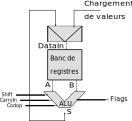
\includegraphics[scale=0.5]{pictures/ALU_Registers.pdf}

Il est ainsi possible de valider leur comportement en enregistrant des données dans le banc de registre (à l'aide des ports \texttt{DataIn} et \texttt{RegDest})
puis en effectuant diverses opération par l'ALU en spécifiant  le \texttt{Codop}.
